% This section is subsubsection crazy and all the whitespace ends up looking absurd.
% If needed, a similar block with the defaults can just be placed at the end of this section though.
% And if people prefer it like this, it can be moved to the preamble.
\titlespacing*{\subsubsection}
{0pt}{1ex}{0ex}


\section{Calibration Products Pipeline (\wbsCPP)}
\label{sec:cpp}

This section details the input data and algorithms required to generate all data products necessary for the photometric calibration of the survey, but does not cover the details of their application.

The various input datasets are covered in \secsymbol\ref{sec:CPP:inputs} and \secsymbol\ref{sec:CPP:auxTelescope:inputs}, which detail the source of the input data, \ie which will be provided by the camera team and which will be measured on the mountain. \secsymbol\ref{sec:CPP:CBP_control} covers miscellaneous algorithms which will be necessary to develop in order to acquire the input datasets with the collimated beam projector (CBP). Finally, sections \secsymbol\ref{sec:CPP:output} and \secsymbol\ref{sec:CPP:auxTelescope:outputs} list the various output data products from the Calibration Products Pipeline.

\subsection{Key Requirements}
\label{sec:CPP:keyRequirements}
The work performed in this WBS serves several complementary roles:

\begin{itemize}
 \item It will enable the production of calibration data products as required by the Level 2 Photometric Calibration Plan (\NewPCP{}) and other planning documents \cite{Lupton15}\footnote{Resolving contradictions between these documents is out of scope here.}. This includes both characterization of the sensitivity of the LSST system (optics, filters and detector) and the transmissivity of, and emission from, the atmosphere;
 
 \item It will characterize detector anomalies in such a way that they can be corrected either by the instrument signature removal routines in the Single Frame Processing Pipeline (\wbsSFM) or, if appropriate, elsewhere in the system;
 
 \item It will provide updated values of the crosstalk matrix to the camera DAQ (for AP) and DM (for DRP) for correction of the raw data;
 
 \item It will allow for characterization of the optical ghosts and scattered light in the system.
\end{itemize}


%%%%%%%%%%%%%%%%%%%%%%%%%%%%%%%%%%%%%%%%%%%%%%%%%%
%%%%%%%%%%%%%%%%%%%%%%%%%%%%%%%%%%%%%%%%%%%%%%%%%%
%%%%%%%%%%%%%%%%%%%%%%%%%%%%%%%%%%%%%%%%%%%%%%%%%%

\subsection{Inputs}
\label{sec:CPP:inputs} 
The following section lists the input datasets which will be available to the Calibration Products Pipeline. It should be noted that these are the raw inputs, and as such, the algorithmic sections for items that are listed as camera team deliverables are shown as ``None'', as these will have been previously derived. However, many of these items are re-listed in the \hyperref[sec:CPP:output]{outputs section}, where the algorithms to recalculate/monitor these on the mountain are detailed.
%\ref{sec:CPP:output}

\subsubsection{Bias Frames}\label{sec:CPP:inputs:biases} 
Sets of bias frames for the production of master biases.
\alg None - these just need to be taken.


\subsubsection{Gain Values}\label{sec:CPP:inputs:gain} 
\cameraTeam
Gain values for all amplifiers; note that these are required to high accuracy (0.1\%), as they are used in determination of the photometric flats.
\alg Measurement is subtle but not hard; both \fefiftyfive\ and PTC gain measurement techniques need to be applied with some care to get good results. Given the \bfeffect\ and non-linearity, it's not clear to what accuracy PTC can give gains, but \fefiftyfive\ can certainly provide gain to $\ll$0.1\% for small signal levels.


\subsubsection{Linearity}\label{sec:CPP:inputs:linearityCurve} 
\cameraTeam
The linearity curve for every amplifier, as well as the level above which these non-linearity curves may be unreliable.
\alg None.


\subsubsection{Darks}\label{sec:CPP:inputs:dark}
Sets of long dark frames (\smalltilde 300s, length TBD based on dark current in delivered sensors) .
\alg None - these just need to be taken.


\subsubsection{Crosstalk}\label{sec:CPP:inputs:crosstalk}
\cameraTeam
The crosstalk matrix for every pair of amplifiers in the camera, though this will likely be a very sparse.
\alg None.


\subsubsection{Defect Map}\label{sec:CPP:inputs:defectList} 
\cameraTeam
A list of all bad (unusable) pixels in each CCD, as well as list of possibly suspect pixels, \ie ones which should be flagged as such during processing.
\alg None.


\subsubsection{Saturation levels}\label{sec:CPP:inputs:saturationLevel}
\cameraTeam
The lowest level (in electrons), for each amplifier, at which charge bleeds to a neighboring pixel. If necessary, they will also provide the level at which the serial register saturates (\ie if the serial saturates at a lower level than the parallels).
\alg None.


\subsubsection{Broadband Flats}\label{sec:CPP:inputs:broadFlat}
Sets of flats taken through the standard LSST filters. We will need flats taken at a number of flux levels to measure brighter-fatter and check linearity, including sets of ``superflats'', which are sets of high-flux flats with many repeats ($>50$, possibly $>100$). Superflats for brighter-fatter characterization will not need to be taken regularly as this effect is not expected to evolve in time.
\alg None - these just need to be taken.


\subsubsection{Monochromatic Flats}\label{sec:CPP:inputs:monoFlat}
Sets of `monochromatic' (\c 1nm) flat-field screen images taken with no filter/glass in the beam.
\alg None - these just need to be taken.


\subsubsection{CBP Data}\label{sec:CPP:inputs:CBP}
Sets of Collimated Beam Projector images. The proposed resolutions and steps in these datasets are preliminary. All the CBP data will be processed using the standard LSST ISR, except that no flat fields will be applied. We will then use standard LSST aperture photometry to measure the number of counts in each CBP spot.
\alg Scripting the CBP/8.4m to take each of these datasets in concert. The scripting/control requirements for the CBP are dealt with separately in \secsymbol\ref{sec:CPP:CBP_control}.


\paragraph{CBP dataset 1}\label{sec:CPP:inputs:CBP:mono}
Sets of CBP images scanned in wavelength at 1nm resolution\footnote{1nm `resolution' here denotes the bandwith of the light source, and can be this width, or any amount lower. It should, however, be noted that the accuracy on the wavelength calibration of the light source needs to be at the 0.1nm level \XXX{Add a reference to the DESC people saying this is necessary for SN cosmology in LSST.}} every 1nm for a fixed set of spot positions on the camera, and for fixed footprint on M1. No filter should be in the beam.
	
	
\paragraph{CBP dataset 2}\label{sec:CPP:inputs:CBP:spot}
Sets of CBP images scanned in wavelength at 20nm bandwidth every 100nm, while rotating the CBP about a pupil to move the spot pattern around the camera for a fixed footprint on M1. No filter should be in the beam.

	
\paragraph{CBP dataset 3}\label{sec:CPP:inputs:CBP:M1}
Sets of CBP images scanned in wavelength at 20nm resolution every 100nm for a fixed set of spot positions on the camera, and for a number of footprints on M1; the minimum number of footprints is \c 6 for a 30cm CBP, but in reality we will explore more pointings to test azimuthal symmetry. No filter should be in the beam.


\paragraph{CBP dataset 4}\label{sec:CPP:inputs:CBP:filter}
Sets of CBP images scanned in wavelength at 1nm resolution every 1nm for a fixed set of spot positions on the camera, and for fixed footprint on M1. Repeated for every filter. \Nb the wavelength range for each scan need only cover the range for which the filter transmits appreciable light.


\paragraph{CBP dataset 5}\label{sec:CPP:inputs:CBP:leak}
Sets of CBP images scanned in wavelength at 20nm resolution every 20nm for a fixed set of spot positions on the camera, and for fixed footprint on M1. Repeated for every filter.


\paragraph {CBP Crosstalk Measurement}\label{sec:CPP:inputs:CBP:crosstalk}
Sets of CBP images taken with a suitably designed sparse mask to allow us identification and measurement of all crosstalk images. The simplest sparse mask would have only a single spot, used to illuminate each amplifier in the camera in turn (but less sparse solutions are likely also possible). The wavelengths used are unimportant, and there are no constraints on beam footprints on M1 or filter choice. This will be particularly necessary should LSST be operated in a slow-readout mode, for example for use with 30s integrations, as crosstalk coefficients would change considerably.


\subsubsection{Filter Transmission}\label{sec:CPP:inputs:filterTransmission}
Transmission curves for all the filters as a function of position. \Nb This is to be delivered by the filter vendors rather than the camera team, but is input data which will not be measured by DM. The resolution needs to be (\XXX{We need to check what the proposed wavelength resolution and accuracy the vendors are proposing to use for this is. I spoke to Steve Ritz at the AHM and he seemed very positive about the vendors proposal for this, but we should check what the plan is.}) 1nm or better, in keeping with the resolution of the monochromatic flats.
\alg None.


\subsubsection{Stellar spectra}\label{sec:CPP:inputs:starSpectrum} 
One or more spectrophotometrically-calibrated spectra star(s) in the field of view for every visit.
\alg How these will be chosen or produced is TBD.


\subsubsection{Other stellar spectra (\nb~!= \ref{sec:CPP:inputs:starSpectrum})}\label{sec:CPP:inputs:standardStarSpectrum}
Known spectra for bright stars in the field of view for all visits.
\alg How these will be chosen or produced is TBD.


\subsubsection{Atmospheric Characterization}\label{sec:CPP:inputs:atmosphericData}
External measurements of atmospheric parameters, \eg the barometric pressure, ozone and temperature.
\alg None, other than interfacing with the site team or parties responsible for the equipment, to automate obtaining the measurements in a machine-readable form, including the ozone data from satellites.


\subsubsection{Photometric Standards}\label{sec:CPP:inputs:photometricStandards} 
A set of photometric standard stars covering a range of colors lying within an appropriate magnitude range. The likely source of this data is GAIA, however, should this prove not to be an appropriate source, a catalog would be carefully generated using the survey's most photometric data, utilizing an \"ubercal/jointcal type approach.
\alg Constructing color transformations from the GAIA measurements, based on assumptions about the objects' intrinsic SEDs, \ie not using only color terms. In the case that GAIA does not provide the catalog, a process similar to the Forward Global Calibration Model implemented by  Eli Rykoff and David Burke for DES would be used. The latter process would likely be able to share atmospheric modeling code with the reductions performed for the \auxtelescope.

%%%%%%%%%%%%%%%%%%%%%%%%%%%%%%%%%%%%%%%%%%%%%%%%%%%%%%%%%%
%%%%%%%%%%%%%%%%%%%%%%%%%%%%%%%%%%%%%%%%%%%%%%%%%%%%%%%%%%
%%%%%%%%%%%%%%%%%%%%%%%%%%%%%%%%%%%%%%%%%%%%%%%%%%%%%%%%%%

\subsection{Outputs from the Calibration Product Pipelines \\
	/ Inputs to the Alert/DRP Pipelines}
\label{sec:CPP:output}

This section details the outputs from the Calibration Products Pipeline. Algorithms for the production of each item are outlined, and includes provision for the re-calculation of items previously only listed as ``camera team deliverables''.

\subsubsection{Master Bias}\label{sec:CPP:output:bias}
Trimmed, overscan subtracted, master bias frame produced by taking the median of several-to-many bias frames for each CCD on the focal plane. \XXX{Including the wavefront sensors?)}
\alg Given the LSST 2s readout, we do not expect to need to remove cosmic rays explicitly; a robust stacking algorithm should be sufficient. A prototype construction algorithm currently exists in \texttt{pipe\_drivers}. Final version must be configurable to use scalar-, vector- or array-type overscan subtraction. 
\footnote{If the readout noise in any channels is too low (relative to the
gain) to properly sample the noise distribution, a simple fix is to add sets of $n$ (\eg 3) bias exposures before creating the stacked image.}


\subsubsection{Master Darks}\label{sec:CPP:output:dark}
Trimmed, overscan and bias-frame subtracted, master dark frames for each CCD on the focal plane. These are produced by taking the median of several-to-many long (c. 300s) dark exposures, and are subsequently scaled to 1 second exposure length.  \XXX{Including the wavefront sensors?)}
\alg The individual frames will be run through standard ISR processing (including cosmic ray removal) before
being combined; the combination may be done using standard LSST image stacking code, and a prototype construction algorithm exists in \texttt{pipe\_drivers}. Final version must be configurable to use scalar-, vector- or array-type overscan subtraction, and be robust to contamination from cosmic rays when coadding.


\subsubsection{Master Linearity}\label{sec:CPP:output:linearityCurve}
Linearity curves; identical to \secsymbol\ref{sec:CPP:inputs:linearityCurve}, unless updated during operations.
\alg Will need to write algorithmic component to generate the linearity curves from raw data, either from binned flats, CBP data or ``ramp frames''. Requires careful treatment as the \bfeffect can masquerade as non-linearity. Code to apply non-linearity correction during \texttt{isr} is currently being implemented by Russell Owen. Care must be taken to calculate these after bias subtraction, or be consistent with the way in which they are applied during ISR.


\subsubsection{Master Fringe Frames}\label{sec:CPP:output:fringeFrames}
Compound (polychromatic) fringe frames, dynamically created to match the emission spectrum of the atmosphere at the time of observation.
\alg Construction of these fringe frames from \hyperref[sec:CPP:output:monoPhotoFlat]{monochromatic flats}, likely using the existing PCA algorithm in \texttt{pipe\_drivers}.


\subsubsection{Master Gain Values}\label{sec:CPP:output:gains}
Per-amplifier gains; identical to \secsymbol\ref{sec:CPP:inputs:gain}, unless updated during operations.
\alg Potentially difficult, and needs to be developed. We will have almost arbitrarily accurate gain measurements as an input, but monitoring the evolution of these gains to the required accuracy is currently an unsolved problem.

We will be able to monitor the relative gain within a given CCD by demanding that the flat fields be continuous across amplifier boundaries; this is, however, more difficult across device boundaries. Ticket \hyperref{https://jira.lsstcorp.org/browse/DM-6030}{}{}{\texttt{DM-6030}} exists to explore the possibility of using cosmic ray muons and the unavoidable radioisotope contamination inside the camera for this purpose. If this fails \footnote{Merlin's estimate is that the likelihood of failure is moderate-to-high, Robert disagrees.} then another method will need to be devised. The necessary accuracy of this measurement should be firmly established.


\subsubsection{Master Defects}\label{sec:CPP:output:defectList}
A list of all bad pixels in each CCD; identical to \secsymbol\ref{sec:CPP:output:defectList}, unless updated during operations.
\alg Perform statistical analysis of dark frames, flats and ``pocket-pumping" exposures to derive an updated defect list.


\subsubsection{Saturation Levels}\label{sec:CPP:output:saturationLevel}
The level (in electrons), for each amplifier, at which charge bleeds to a neighboring pixel; identical to \secsymbol\ref{sec:CPP:output:saturationLevel}, unless updated during operations.
\alg Measured using the CBP if the spots are well-formed and stable. If not, measured by saturating many stars in long sky exposures and dithering, with custom processing to calculate the PSF from the unsaturated stars. Development of code to detect where saturation is occurring, and subsequently calculate the saturation levels.


\subsubsection{Crosstalk}\label{sec:CPP:output:crosstalk}
The crosstalk matrix element for every pair of amplifiers in the camera; identical to \secsymbol\ref{sec:CPP:output:crosstalk}, unless updated during operations. The probability that we'll need to update is high as the validity of these values depends on them being measured with the camera in its final configuration. The reasoning is that the inter-CCD and inter-raft couplings, though supposedly small (especially in the case of inter-raft coupling), depend on the exact physical locations of all the circuit boards and flex cables with respect to one another. We must therefore be able to measure this on the mountain using the CBP.
%\XXX{Remove this commentary in final version:} Whilst this is not ``hard'' in the intellectual sense, it is a fiddly thing and easy to get wrong, both in the measurement and potentially the correction; the LSST focal plane is likely to be heterogeneous, and the readout direction between the amplifiers differ between the chip flavors, meaning that crosstalk ghosts may appear mirrored in one or more axes. Furthermore, whilst unlikely to exist (nay certain, we are assured), \emph{should} a timing offset exist between REBs or CCDs, the crosstalk ghost positions would change, and a single matrix would be insufficient to describe the correction.
\alg In the un-multiplexed limit, this involves dithering a single CBP spot around the focal plane and measuring the crosstalk ghosts (whilst carefully disambiguating these from optical ghosts using CBP trickery). Clearly some multiplexing will be possible using a multi-pinhole CBP mask. We should baseline for a one-spot-per-CCD mask, a one-spot-per-raft-mask, and ideally a one-spot-per-amplifier mask, as well as a single-spot mask.

CBP dithering scripts will be written which will involve mask-specific raster scanning routines, followed by either performing a camera rotation or by re-raster scanning at a different M1 position for the previous focal plane positions to differentiate crosstalk and optical ghosts. Code to perform this differentiation will be written, which will then make the measure the coupling coefficients. Further reading on crosstalk in LSST CCDs can be found in \cite{OConnor15},

Confirmation of the measured crosstalk matrix will be performed using either CBP data, saturated stars' bleed trails, or cosmic rays in dark frames.
%\begin{note}
%	See queries on crosstalk which I have put in \secsymbol\ref{sec:calibQuestions}.
%\end{note}



\subsubsection{Impure Monochromatic Flats}\label{sec:CPP:output:monoFlat}
Sets of `monochromatic' (\c 1nm) trimmed, overscan-subtracted, dark-corrected flat-field images for each filter. These flats will \emph{include} ghost and scattered light.
\alg Construction algorithm exists in \texttt{pipe\_drivers}.


\subsubsection{Pure Monochromatic Flats}\label{sec:CPP:output:monoPhotoFlat}
Sets of `monochromatic' (\c 1nm) trimmed, overscan-subtracted, dark-corrected flat-field images for each filter. These flats will \emph{exclude} ghost and scattered light.
\alg Constructed from \secsymbol\ref{sec:CPP:output:monoFlat} and corrected using 2D spline fits to the photometric measurements of the CBP spots. See \XXX{cite RHL here} for further reading.


\subsubsection{PhotoFlats}\label{sec:CPP:output:standardPhotoFlat}
The linear combination of \secsymbol\ref{sec:CPP:output:monoPhotoFlat} data weighted by a flat-spectrum source (or other defined standard SED), absorbed by a standard atmosphere, and observed through each filter.
\alg Combining \secsymbol\ref{sec:CPP:output:monoPhotoFlat} should be simple; need to define the ``standard atmosphere'' and ``standard SED''.


\subsubsection{Low-res narrow-band flats}\label{sec:CPP:output:monoPhotoFlatLowRes}
A low-resolution (in both space and wavelength) version of \secsymbol\ref{sec:CPP:output:monoPhotoFlat}.
\alg Scripting to perform the necessary sweeps of the laser light source, and characterization of its output as the pulse energy will likely need to be normalized to.	


\subsubsection{Pixel Sizes}\label{sec:CPP:output:pixelSizeMap} 
A map of the (effective) pixel-size distortions. At worse, this will be a $n_{\mbox{width}}\times n_{\mbox{height}}\times 2$ datacube of floats. Pixel size distortions include small-scale quasi-random size variations, mask-stitching/tiling artifacts, tree-rings, and any other effects not dynamical in nature.
\alg Algorithm to measure this is currently a (somewhat) unsolved problem. It has been claimed by Aaron Roodman \& co. that these can be measured from flat-fields, but the problem is under-constrained, and thus the stability (nay, validity?) of their measurements is questionable, despite seeming to work. Further thought is required to establish whether their method can be used, and if not, devise another one (though it is not obvious how the problem can be made to be well constrained). 
\\ \dragons ?


\subsubsection{Brighter-Fatter Coefficients}\label{sec:CPP:output:brighterFatterCoeffs}
Coefficients needed to model the brighter-fatter effect. We hope that these are a small number of floats per CCD, but this is not yet entirely clear. The input data necessary to calculate these will likely be restricted to \hyperref[sec:CPP:inputs:broadFlat]{superflats} at various flux levels, with the possible addition of some star fields for verification of the coefficients.
\alg A number of techniques exist to measure these (mostly developed by members of the DESC SAWG). Code already exists to estimate the kernel/coefficients, and apply the corrections using an enhanced version of the Astier/Antilogus technique.
\\ \dragons ?


\subsubsection{CTE Measurement}\label{sec:CPP:output:CTE}
\XXX{Rewrite this section}
Measurement of the charge transfer efficiency for each amplifier/column in the camera. In the most simplistic case this would be a single number per amplifier, but this case is the worst for science as it means the dominant trap is in the close to the amplifier in the serial register and thus affects all columns equally. At worst with respect to data-product size (or at best for science) this is a number per column in the simple case, though one could imagine characterizing the specific defects and their locations on the chips, in which case this is a per-pixel product (though could be simplified using bounding-boxes as with defect maps). The nominal case should be considered as per-column. Furthermore, if the number of columns with significant effects is small, these columns would most likely be masked out rather than corrected.
\alg Measurement of CTE is subtle, but not hard, and several established methods exist for doing this. Using the \fefiftyfive method won't be possible due to the lack of a radioisotope source in the camera, but the flat-field overscan excess measurement method and flat-field correlation method would both be possible using existing input data products. See \XXX{} for further reading on these methods, one of which would need to be implemented within the DM framework.
%\begin{note}[Backport to RHL's doc]
%	CTE measurement and correction sections needs to be added to RHL's calibration documents. This is looking like it may not be a negligible effect for photometry, astrometry and shape measurement, and I don't think it's currently mentioned anywhere in those.
%\end{note}


\subsubsection{Filter Transmission}\label{sec:CPP:output:filterTransmission}
Monitoring of filter transmission \emph{in-situ}. As well as the filter transmission measurement from the camera team/vendor in \secsymbol\ref{sec:CPP:inputs:filterTransmission}, we further baseline the development of a procedure for monitoring the filter response at 1\,nm resolution using the approach described in \cite{Lupton15}, \ie by making suitable CBP measurements with and without the filter in the beam, doing averaging over the angles.
\alg Created from measurements in \secsymbol\ref{sec:CPP:inputs:CBP}.


\subsubsection{Ghost catalog}\label{sec:CPP:output:GhostCatalog}
A catalog of optical ghosts and glints which is available for use in other parts of the system. Detailed characterization of ghosts in the LSST system will only be possible when the system is operational. Our baseline design therefore calls for this system to be prototyped using data from precursor instrumentation; we note that ghosts and ghoulies in \eg HSC are well known and more significant than are expected in LSST.
\begin{note}
It is not currently clear where the responsibility for characterizing ghosts and glints in the system lies. We assume it is outside this WBS. RHL instructed to note that this is a possible new entry to the risk registry.
\end{note}



%%%%%%%%%%%%%%%%%%%%%%%%%%%%%%%%%%%%%%%%%%%%%%%%%%%%%%%%%%
%%%%%%%%%%%%%%%%%%%%%%%%%%%%%%%%%%%%%%%%%%%%%%%%%%%%%%%%%%
%%%%%%%%%%%%%%%%%%%%%%%%%%%%%%%%%%%%%%%%%%%%%%%%%%%%%%%%%%


\subsection{CBP Control}\label{sec:CPP:CBP_control}
The procurement of the CBP includes the procurement of the necessary low-level control drivers/software. T\&S TCS own the task of taking the vendor-provided low-level routines and turning these into real-world usable routines (higher level functions for \eg homing, slew-to-position, mount requested filter \etc.)

However, it will still remain to write scripts for the CBP, and interfaces with the OCS, to allow making all of the desired measurements, especially as several of these, namely \xxx, \xxx \& \xxx require doing so in concert with the 8.4m.
\alg As well as writing the necessary scripts to acquire the raw data products outlined in \secsymbol\ref{sec:CPP:inputs}, it will also be necessary to deliver the coordinate transformation and pointing model to allow the CBP to maintain a fixed position on the focal plane whilst illuminating different portions of the pupil (and vice versa.)
















%%%%%%%%%%%%%%%%%%%%%%%%%%%%%%%%%%%%%%%%%%%%%%%%%%%%%
%%%%%%%%%%%%%%%%%%%%%%%%%%%%%%%%%%%%%%%%%%%%%%%%%%%%%
%%%%%%%%%%%%%%%%%%%%%%%%%%%%%%%%%%%%%%%%%%%%%%%%%%%%%


\subsection{Calibration Telescope Input Calibration Data}
\label{sec:CPP:auxTelescope:inputs}
This section details the input data required to calibrate the \auxtelescope itself. Broadly, this will include most of the ingredients listed in \secsymbol\ref{sec:CPP:inputs}, but namely:

\begin{itemize}
	\item Gain values \footnote{Less accuracy is needed here than for the main camera; a PTC-based measurement will be sufficient.}
	\item Crosstalk matrix
	\item Linearity curves for each amplifier
	\item Defect map
	\item Saturation levels
	\item Bias frames
	\item Dark frames
	\item Broadband flat-fields
	\item Narrowband flat-fields\footnote{ It is confirmed to be part of the baseline design that there will be both broadband and narrowband light sources at the \auxtelescope.}.
	\item Filter/grating/grism transmissions
\end{itemize}

Further to these standard camera calibration data products, an illumination/ghost correction will also be required, which will either be derived from star field observations or using the final CBP prototype for direct measurement.


%%%%%%%%%%%%%%%%%%%%%%%%%%%%%%%%%%%%%%%%%%%%%%%%%%%%%
%%%%%%%%%%%%%%%%%%%%%%%%%%%%%%%%%%%%%%%%%%%%%%%%%%%%%
%%%%%%%%%%%%%%%%%%%%%%%%%%%%%%%%%%%%%%%%%%%%%%%%%%%%%





\subsection{Calibration Telescope Output Data}
\label{sec:CPP:auxTelescope:outputs}
This section details the calibrated outputs from the \auxtelescope, which, like items in section \secsymbol\ref{sec:CPP:output}, are output from to the Calibration Products Pipelines to be used in photometric calibration at various levels.


\subsubsection{Atmospheric Absorption}\label{sec:CPP:aux:atmosphericAbsorption}
As shown in Figure~\ref{fig:aux_telescope}, the determination of the atmospheric transmission starts with a two images, one dispersed and one direct, acquired back-to-back with the \auxtelescope, where the camera rotator has been set to align the spectra with the parallactic angle. A scaled version direct image is subtracted from the dispersed image, with the scaling factor governed by the geometric efficiency of the disperser in the beam, resulting in the removal of the zeroth order light, and leaving only the spectra. Regions in which the spectra fall are identified, and the strongest lines in these crude uncorrected-spectra are identified and used to determine the incident wavelength as function of position on the detector. This information is then used in conjunction with the system throughput data-cube to correctly flat-field the dispersed images.

\begin{figure}
	\centering
	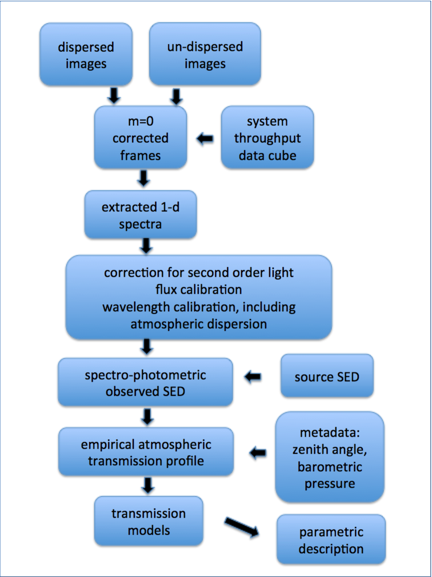
\includegraphics[width=\textwidth]{figures/aux_telescope_workflow.png}
	\caption{Flowchart depicting a summary of the atmospheric absorption determination pipeline.}.
	\label{fig:aux_telescope}
\end{figure}

The 1D spectra are then extracted from the image, flux calibrated, and corrected for second order light contamination. A more precise wavelength calibration is then performed using the spectral lines in this corrected spectrum, taking into account the effect of differential chromatic refraction, resulting in a spectrophotometrically calibrated measurement.

The source's true SED and the calibrated spectrophotometric observation are then used in conjunction with the observational meta-data, \eg the zenith angle, temperature and barometric pressure, to derive an empirical measurement of the atmospheric transmission. This measurement is then matched to atmospheric models to provide a parametric description of the state of the atmosphere at the time of observation.


%\XXX{Add here about how you flat field a dispersed image. (flat fielding is tricky.  Find the 0-order image.  Subtract a (scaled) direct image without flat fielding either dataset.  Construct a flat from monochromatic flats, knowing what wavelength falls where.  flatfield.)}
%The atmospheric absorption as a function of wavelength (at moderate spectral resolution) for almost each visit.
%\alg Broadly speaking, exposures are calibrated using the input data products in \secsymbol\ref{sec:CPP:auxTelescope:inputs}, using a variant of the standard processing pipeline (bias subtraction, flat-fielding, CR rejection \etc). Spectrophotometry is then performed by fitting and measuring the spectra of bright stars in these dispersed images. Then, by comparing these extracted spectra with the known spectrum of each source (or using a bootstrapping technique if the necessary population of calibrated standards does not exist) the atmospheric extinction as a function of wavelength is obtained for that visit.
%
%Further implementation details/refinement will likely include the addition of \hyperref[sec:CPP:inputs:atmosphericData]{barometric pressure and ozone data and temperature}, as well as fitting the measured spectrum to an atmospheric modeling framework \eg MODTRAN, extended to handle a variable aerosol index. \XXX{Probably insert a citation here, and/or mention Stubbs/Guyonet.}


 
\subsubsection{Night Sky Spectrum}\label{sec:CPP:aux:nightSkySpectrum}
Although the acquisition of a night sky spectrograph is uncertain, in the eventuality that we obtain the instrument, we provision for the determination of the emission spectrum of the night sky near the \auxtelescope boresight, with $R \sim 200$\footnote{It is not entirely clear yet whether these will be taken on the Calypso or 8.4m boresight.}, which will be used to synthesize flat-field images matching the sky's SED from the \hyperref[sec:CPP:output:monoFlat]{monochromatic dome flats}.
\alg Assuming we have a sky spectrograph this is simple. In the absence of a sky spectrograph, an $R \sim 10$ spectrum will be acquired using standard/narrowband filters.








%%%%%%%%%%%%%%%%%%%%%%%%%%%%%%%%%%%%%%%%%%%%%%%%%%%%%
%%%%%%%%%%%%%%%%%%%%%%%%%%%%%%%%%%%%%%%%%%%%%%%%%%%%%
%%%%%%%%%%%%%%%%%%%%%%%%%%%%%%%%%%%%%%%%%%%%%%%%%%%%%

\subsection{Prototype Implementation}
\label{sec:CPP:prototypeImplementation}
While parts of the Calibration Products Pipeline have been prototyped by the LSST Calibration Group (see the \NewPCP for discussion), these have not been written using LSST Data Management software framework or coding standards. We therefore expect to transfer the know-how, and rewrite the implementation.











%%%%%%%%%%%%%%%%%%%%%%%%%%%%%%%%%%%%%%%%%%%%%%%%%%%%%
%%%%%%%%%%%%%%%%%%%%%%%%%%%%%%%%%%%%%%%%%%%%%%%%%%%%%
%%%%%%%%%%%%%%%%%%%%%%%%%%%%%%%%%%%%%%%%%%%%%%%%%%%%%

%\subsection{Overview of calibration procedure}
%This section, whilst not strictly concerning the \emph{production} of the calibration products themselves, aims to give a broad overview of how these products will be used and why. 
%\begin{note}
%Whilst this isn't technically part of the CPP remit, without it, all that is here is a list of ingredients, (and how to make the compound ingredients), with no overview of the recipe, which makes for a strange section in a cookbook. If this is no desired or should live somewhere else then feel free to move or \emph{re}move it, but I felt like it should be in here as this stuff is not easy to get ones head around at the best of times.
%\end{note}
%
%\XXX{Overview goes here!}

%\paragraph{Instrumental sensitivity}
%
%
%
%
%\begin{enumerate}
% \item{Record bias/dark frames;}
% \item{Use ``monochromatic'' (1\,nm) flat field screen flats with no filter in the beam to measure the per-pixel sensitivity;}
% \item{Use a collimated beam projector (CBP) to measure the quantum efficiency (QE) at a set of points in the focal plane, dithering those points to tie them together;}
% \item{Combine the screen and CBP data to determine the broad band (10--100\,nm) QE of all pixels;}
% \item{Fold in the filter response to determine the 1\,nm resolution effective QE of all pixels.}
%\end{enumerate}
%
%This WBS is responsible for the development of the data analysis algorithms and software required and the ultimate delivery of the flat fields. Development and commissioning of the CBP itself, together with any other infrastructure required to perform the above procedure, lies outwith Data Management (see 04C.08 \emph{Calibration System}).
%
%\paragraph{Atmospheric transmissivity}
%
%Measurements from the auxiliary instrumentation---to include the 1.2\,m ``Calypso'' telescope, a bore-sight mounted radiometer and satellite-based measurement of atmospheric parameters such as pressure and ozone---will be used to determine the atmospheric absorption along the line of sight to standard stars. The atmospheric transmission will be decomposed into a set of basis functions and interpolated in space in time to any position in the LSST focal plane.
%
%This WBS will develop a pipeline for accurate spectrophotometric measurement of stars with the auxiliary telescope. We expect to repurpose and build upon publicly available code e.g.\ from the PFS\footnote{Subaru's Prime Focus Spectrograph; \url{http://sumire.ipmu.jp/pfs/}.} project for this purpose.
%
%This WBS will construct the atmospheric model, which may be based either on \textsc{modtran} (as per \NewPCP{}) or a PCA-like decomposition of the data (suggested by \cite{Lupton15}).
%
%This WBS will define and develop the routine for fitting the atmospheric model to each exposure from the calibration telescope and providing estimates of the atmospheric transmission at any point in the focal plane upon request.
%
%\paragraph{Detector effects}
%
%An initial cross-talk correction matrix will be determined by laboratory measurements on the Camera Calibration Optical Bench (CCOB). However, to account for possibile instabilities, this WBS will develop an on-telescope method. We baseline this as being based on measurement with the CBP, but we note the alternative approach based on cosmic rays adopted by HSC \cite{Furusawa14}.
%
%Multiple reflections between the layers of the CCD give rise to spatial variability with fine scale structure in images which may vary with time \cite[\S2.5.1]{Lupton15}. These can be characterized by white light flat-fields. Preliminary analysis indicates that these effects may be insignificant in LSST \cite{Rasmussen15}; however, the baseline calls for a routine developed in this WBS to analyse the flat field data and generate fringe frames on demand. This requirement may be relaxed if further analysis (outside the scope of this WBS) demonstrates it to be unnecessary.
%
%
%This WBS will develop algorithms to characterize and mitigate anomalies due to the nature of the camera's CCDs.
%
%\begin{note}
%There's a complex inter-WBS situation here: the actual mitigation of CCD anomalies will generally be performed in SFM (\wbsSFM{}), based on products provided by this WBS which, in turn, may rely on laboratory based research which is broadly outside the scope of DM\@. We baseline the work required to develop the corrective algorithms here. We consider moving it to \wbsSFM{} in future.
%\end{note}
%
%The effects we anticipate include:
%
%\begin{itemize}
% \item{QE variation between pixels;}
% \item{Static non-uniform pixel sizes (e.g.\ ``tree rings'' \cite{Stubbs14});}
% \item{Dynamic electric fields (e.g.\ ``brighter-fatter'' \cite{Antilogus14});}
% \item{Time dependent effects in the camera (e.g.\ hot pixels, changing cross-talk coefficients);}
% \item{Charge transfer (in)efficiency (CTE).}
%\end{itemize}
%
%Laboratory work required to understand these effects is outwith the scope of this WBS\@. In some cases, this work may establish that the impact of the effect may be neglected in LSST\@. The baseline plan addresses these issues through the following steps:
%
%\begin{itemize}
% \item{Separate QE from pixel size variations\footnote{Refer to work by Rudman.} and model both as a function of position (and possibly time);}
% \item{Learn how to account for pixel size variation over the scale of objects (e.g.\ by redistributing charge);}
% \item{Develop a correction for the brighter-fatter effect and develop models for any features which cannot be removed;}
% \item{Handle edge/bloom using masking or charge redistribution;}
% \item{Track defects (hot pixels);}
% \item{Handle CTE, including when interpolating over bleed trails.}
%\end{itemize}
%


%

%Produce Master Pupil Ghost Exposure; Determine CCOB-derived Illumination Correction; Determine Optical Model-derived Illumination Correction; Determine Star Raster Photometry-derived Illumination Correction; Create Master Illumination Correction; Determine Self-calibration Correction-Derived Illumination Correction; Correct Monochromatic Flats; Reduce Spectrum Exposure


%%%%%%%%%%%%%%%%%%%%%%%%%%%%%%%%%%%%%%%%%%%%%%%%%%%%%
%%%%%%%%%%%%%%%%%%%%%%%%%%%%%%%%%%%%%%%%%%%%%%%%%%%%%
%%%%%%%%%%%%%%%%%%%%%%%%%%%%%%%%%%%%%%%%%%%%%%%%%%%%%

%\subsection{UNSTRUCTURED OPEN QUESTIONS \\ a.k.a. Merlin's random thoughts/ramblings}\label{sec:calibQuestions}

%This section is just things that I thought of whilst working through this document. They probably don't belong in here at all, but I wanted to capture them and this seemed a semi-relevant place (and Jim started it!).
%\begin{itemize}
%	\item Flat fielding the auxiliary telescope: What is required? What are the plans? We have a flat-field screen in this dome, correct? (Now confirmed) Regarding the bandpasses, what do we have in terms of filters? (Answer: full LSST set on the imager) What do we need? Is it not necessary get an accurate throughput determination at 1nm resolution by taking the CBP or at least the monochromatic laser source over there for a one-off characterization? (Answer: the laser is not going to happen but there is a monochromatic light source in the \auxtelescope\ baseline.) If not, how are we accurately characterizing the response of the detector which will itself be doing the $R \sim 200$ spectrophotometry of the standard stars?
%	\begin{note}
%		Need to go back and add in doing monochromatic composite flat-fielding of this telescope, \emph{and} add that these need to be applied somewhere/somehow. The application of \emph{these} to the \auxtelescope\ data really doesn't belong in AP or DRP as all the other photocal stuff does.
%	\end{note}
	
%	\item Crosstalk coupling: depending on where this happens in the electronic chain, this may be ``conservative" or ``generative", \ie\ if the crosstalk is from a capacitive coupling at an early stage of the readout then the crosstalk which is removed from the victims should be added back in to the aggressors, as this is signal which has been \emph{lost}. However, if it occurs after a significant amount of amplification (likely), then it should just be removed. Again, I'm sure this is known but I'd just like to check as this matters at the sub 1\% level. \rednote{Answer: Very likely generative, but the reasoning for this assumes a low impedance on the output analog lines (such that the voltage does not drop when capacitive coupling occurs) but this is actually not necessarily the case, and perhaps should be checked more thoroughly. Can likely persuade Paul O'Connor/Andrei Nomerotski/Hyeyun Park to investigate if necessary.}
	
%	\item Crosstalk (again): I am lead to believe that crosstalk correction will be applied in the DAQ. If this is correct, then this point is just to note that the calibration system needs to be able to disable this and access the truly raw images in order to make the crosstalk matrix measurements using CBP spots. It will also need to be able to push a new crosstalk matix to the DAQ to confirm meaurements (and to update the system in general). \rednote{RHL says this is already captured somewhere relevant.}
	
%	\item Crosstalk (yet again): Has anyone considered the nightmare scenario where crosstalk is a function of alt, az and rotator position due to changes in these couplings from cable movement? Or is this certain to be only a 1\% change in a 1\% effect, and therefore not a concern? \rednote{Answer: Turns out that it really is very unlikely indeed, as almost everything comes from intra-flex-cable coupling and wire-bond coupling, which won't move when the camera is repositioned.}
	
%	\begin{note}
%		Need to include algorithm for applying crosstalk corrections after the fact in the event that the data-buffer overflows in the case of internet outages between the summit and the US. The also implies that a time history of the measured crosstalk matrices needs to be stored somewhere.
%	\end{note}
		
%	\item Does bleeding occur only in the serial register? (surely not) If not then why do we expect it to be a per-amplifier thing particularly, rather than a per pixel effect, as it is presumably defined by the depth of each well? This is surely known, but I should discuss with someone. \rednote{Answer: There is more than one thing here: bleeding/blooming $\neq$ saturation. Blooming levels are a per-pixel effect (though likely very similar throughout a chip), whilst ``saturation'' is in the amplifier/ADC, which is obviously per-channel. }
	
%	\item Pulse-to-pulse variation in the narrowband laser. When averaged over, what is the RMS? And how stable is the mean over time? (I have met lasers which drift \bfeffect{like crazy}). How do these properties change as one sweeps the wavelength around as would be required for taking the 20nm width flats?
	

%\end{itemize}



\subsection{Miscellaneous Algorithms}\label{sec:CPP:miscAlg}
\begin{itemize}
	\item CBP image processing:
		\mysubitem Starflat like processing to solve for spot brightnesses
		\mysubitem Optical ghost / crosstalk disambiguation
		\mysubitem Derivation of ghosting model? (perhaps not in the WBS)
%		\mysubitem Control
	\item Photometric flat construction from CBP pointings. Roughly:
		  \mysubitem Having performed starflat-like processing, and normalized to the results, fit a surface through the CBP values (either per-CCD or for the whole camera); a spline would be a reasonable choice (either the product of two 1-D splines, or a thin plate spline. RHL would start with the former as they are easier to understand).
		  \mysubitem Divide the dome flat by this surface, giving an estimate of the illumination and chip-to-chip correction
		  \mysubitem Fit a curve to this correction, and correct the dome screen.  This should be close to the values derived from the CBP data (and can preserve discontinuities in the QE across chips which the fitted curves have a hard time following).
		  \mysubitem Iterate a couple of times; each iteration should result in a smaller and smoother correction, which we are therefore better able to model.
		  \mysubitem Then repeat the above at a suitable set of wavelengths, chosen so that the variation of these corrections as a function of wavelength is well captured; we now know the the relative QE for all pixels in the camera, as a function of wavelength, in the absence of a filter.
		  \mysubitem Using the filter transmission curves we can then derive the relative QE for all pixels in the camera for each filter at 1nm resolution; this is our monochromatic photometric flatfield.
	 \item Ghosting model: Following the above analysis we will have information which, whilst not needed to perform the calibration of LSST, will provide a valuable cross-check, and will inform the camera and telescope teams about the state of the optical elements, and is therefore an output of the Calibration Products Pipeline. The can be done in two ways:
		  \mysubitem By analysis of the CBP data, concentrating not on the spots but on the scattered/ghost light
		  \mysubitem By looking at the corrections applied to the CBP spot data to arrive at the dome screen data

	
\end{itemize}


\clearpage































%%%%%%%%%%%%%%%%%%%%%%%%%%%%%%%%%%%%%%%%%%%%%%%%%%%
%%%%%%%%%%%%%%%%%%%%%%%%%%%%%%%%%%%%%%%%%%%%%%%%%%%
%%%%%%%%%%%%%%%%%%%%%%%%%%%%%%%%%%%%%%%%%%%%%%%%%%%



%\section{Photometric Calibration Pipeline (\wbsPhotoCal)}
%
%\subsection{Key Requirements}
%
%The Photometric Calibration Pipeline is required to internally calibrate the relative photometric zero-points of every observation, enabling the Level 2 catalogs to reach the required SRD precision.
%
%\subsection{Baseline Design}
%
%The adopted baseline algorithm is a variant of ``ubercal'' \cite{Padmanabhan08, Schlafly12}. This baseline is described in detail in the Photometric Self Calibration Design and Prototype Document (\UCAL).
%
%\subsection{Constituent Use Cases and Diagrams}
%
%Perform Global Photometric Calibration;
%
%\subsection{Prototype Implementation}
%
%Photometric Calibration Pipeline has been fully prototyped by the LSST Calibration Group to the required level of accuracy and performance (see the \UCAL document for discussion). % RHL really? I thought that they wrote a small-scale toy version. But I may be totally out of date.
%\\
%
%As the prototype has not been written using LSST Data Management software framework or coding standards, we assume a non-negligible refactoring and coding effort will be needed to convert it to production code in LSST Construction.
%
%\clearpage
%
%\section{Astrometric Calibration Pipeline (\wbsAstroCal)}
%
%\subsection{Key Requirements}
%
%The Astrometric Calibration Pipeline is required to calibrate the relative and absolute astrometry of the LSST survey, enabling the Level 2 catalogs to reach the required SRD precision.
%
%\subsection{Baseline Design}
%
%Algorithms developed for the Photometric Calibration Pipeline (\wbsPhotoCal) will be repurposed for astrometric calibration by changing the relevant functions to minimize. This pipeline will further be aided by WCS and local astrometric registration modules developed as a component of the Single Frame Processing pipeline (\wbsSFM).
%\\
%
%Gaia standard stars will be used to fix the global astrometric system. It is likely that the existence of Gaia catalogs may make a separate Astrometric Calibration Pipeline unnecessary.
%
%\subsection{Constituent Use Cases and Diagrams}
%
%Perform Global Astrometric Calibration;
%
%\subsection{Prototype Implementation}
%
%The Astrometric Calibration Pipeline has been partially prototyped by the LSST Calibration Group, but outside of LSST Data Management software framework. We expect to transfer the know-how, and rewrite the implementation.
